\chapter{팽창하는 우주의 기하학}

여기서 다루는 것은 팽창하는 우주와 그 기하학이다. 팽창을 일으키는 요인을 묻기에 앞서 공간이 팽창한다는 것이 무엇을 뜻하는지 설명하는 것이 목표다. 뉴턴 역학의 \(F=ma\) 우주론은 나중에 다루며, 그 뒤에야 기하학과 동역학을 합쳐 완전한 프리드먼--로버트슨--워커 체계를 구성한다.

\section{팽창하는 직선 위의 공변 좌표}

가능한 한 단순한 예인 시공간이 아닌 1차원 공간에서 시작하자. 은하들이 일정한 간격으로 놓인 무한한 직선을 상상해 보자. 좌표 \(x\)는 아직 물리적 거리를 재지 않는다. 은하에 이름표를 붙일 뿐이다. \(x\)를 은하의 이름이라고 생각해도 좋다. 배열 전체가 늘어나거나 줄어들더라도 그 이름은 은하에 계속 붙어 있다.

\(x=0\)라고 불리는 은하에서 \(x=1\)이라고 불리는 은하까지의 물리적 거리를 \(a\)라고 하자. 그러면 임의의 두 은하 사이의 물리적 거리는
\begin{equation}
d=a\,\Delta x.
\end{equation}
좌표 차이 \(\Delta x\)는 이름표 사이의 차이일 뿐이다. 인자 \(a\)는 그 이름표 차이를 미터자로 잰 실제 거리로 바꿔 준다.

이제 직선이 늘어나는 탄성 실이라고 상상해 보자. 이름표는 은하에 붙어 있지만, 이웃 은하 사이의 거리는 시간에 따라 변한다. 같은 관계식은 다음과 같이 된다.
\begin{equation}
d(t)=a(t)\,\Delta x.
\end{equation}
이 단계에서 균질성이란 공통 간격이 시간에 따라 변할 수는 있어도 이웃 은하들이 어디서나 같은 간격으로 떨어져 있다는 뜻일 뿐이다.

\section{허블 법칙과 중심의 부재}

고정된 두 은하의 상대 속도를 구하려면 두 은하를 고정해 \(\Delta x\)가 시간에 따라 변하지 않게 하자. 미분하면
\begin{align}
\dot d &= \dot a\,\Delta x \\
       &= \frac{\dot a}{a}\,a\,\Delta x \\
       &= \frac{\dot a}{a}\,d.
\end{align}
이제 다음과 같이 정의하면
\begin{equation}
H(t)\equiv \frac{\dot a}{a},
\end{equation}
다음 관계를 얻는다.
\begin{equation}
\dot d = H(t)\,d.
\end{equation}
이것이 허블 법칙이다.

역사적으로 쓰인 ``허블 상수''라는 표현은 오해를 부른다. 이 양은 시간에 대해서가 아니라 공간에 대해 일정하다. 주어진 순간에는 모든 은하에서 같지만, 일반적으로 우주가 진화함에 따라 변한다. 허블 매개변수라고 부르는 편이 더 적절하다.

이 법칙에 따르면 더 멀리 있는 은하일수록 더 빠르게 멀어진다. 하지만 이 법칙은 어떤 중심도 특정하지 않는다. 논의의 어떤 부분도 \(x=0\)나 다른 어느 점도 특별하게 취급하지 않는다. 모든 관측자는 같은 법칙을 본다. 따라서 이 모형의 팽창하는 우주는 특별히 지정된 한 장소에서 일어난 폭발이 아니다.

적색편이는 곧바로 등장한다. 서로 멀어지는 두 은하가 빛 신호를 주고받으면, 수신된 빛은 적색편이를 겪는다. 후퇴 속도가 클수록 적색편이도 크다. 따라서 스펙트럼선은 후퇴 속도에 관한 정보를 알려 준다. 거리를 재기는 더 어렵고, 허블의 초기 추정치는 거칠었다. 그의 첫 그래프는 완벽한 직선이 아니라 불확실성이 큰 점들이 흩어져 있는 그래프였다. 그래도 잡음 속에서 기하학적 원리는 살아남았다. 후퇴 속도는 거리에 비례한다.

\begin{classroomqa}\audiencequestion{은하들이 충분히 멀리 떨어져 있으면 허블 법칙에 따라 광속보다 빠르게 움직이나요?}\lecturetimestamp{00:20:23}\lecturerresponse{네, 이 후퇴의 의미에서는 그렇습니다. 하신 말씀은 맞습니다. 이 문제는 꼭 다시 다루겠습니다. 가장 중요한 내용 가운데 하나입니다.}\end{classroomqa}

\section{고차원, 등방성, 그리고 \(a(t)\)의 시간 의존성}

공간 차원을 더해도 본질적으로 달라지는 것은 없다. 2차원에서는 \((x,y)\)로 표시한 은하들의 정사각 격자를, 3차원에서는 \((x,y,z)\)로 표시한 격자를 상상해 보자. 여기서도 좌표는 동행하는 이름표다. 좌표는 물리적 거리를 직접 재는 대신 은하와 함께 움직인다.

\(x\) 방향의 간격과 \(y\) 방향의 간격이 같아야 하는 이유는 무엇일까? 답은 관측에 있다. 은하들이 한 방향에서 체계적으로 더 빽빽하다면 하늘은 방향에 따라 다르게 보일 것이다. 충분히 큰 규모에서는 그렇지 않다. 이처럼 방향에 따라 달라지지 않는 성질이 등방성이다.

2차원에서 두 은하 사이의 거리는
\begin{equation}
d=a\sqrt{(\Delta x)^2+(\Delta y)^2},
\end{equation}
3차원에서는
\begin{equation}
d=a\sqrt{(\Delta x)^2+(\Delta y)^2+(\Delta z)^2}.
\end{equation}
고정된 은하 쌍에서는 좌표 차이가 일정하므로, 다시 미분하면
\begin{equation}
\dot d=\frac{\dot a}{a}\,d.
\end{equation}
허블 법칙은 그대로다.

균질성은 장소에 따른 동일성을 뜻한다. 등방성은 방향에 따른 동일성을 뜻한다. 어느 쪽도 작은 규모에서 정확히 성립하지는 않는다. 은하수를 바라보는 것과 그 원반 바깥을 바라보는 것은 다르고, 개별 은하들도 짧은 거리 규모에서는 균일하게 퍼져 있지 않다. 그러나 많은 은하에 대해 평균을 내면 큰 규모의 우주는 대략 어디서나, 어느 방향으로나 비슷해 보인다.

\begin{classroomqa}\audiencequestion{속도가 거리에 비례하고 거리가 늘어나고 있다면, 고정된 한 쌍의 은하들은 서로 가속하며 멀어지는 건가요?}\lecturetimestamp{00:40:22}\lecturerresponse{아닙니다. 허블 법칙은 주어진 순간의 후퇴 속도가 거리에 비례한다고 말합니다. 고정된 한 쌍의 은하 사이 속도가 시간에 따라 증가하는지 감소하는지는 그 자체로 말해 주지 않습니다. 그것은 \(a(t)\)의 구체적인 시간 의존성에 달려 있습니다. \(a(t)\propto t\)이면 이웃 은하들은 일정한 속도로 멀어집니다. \(a(t)\propto t^2\)이면 고정된 은하 쌍의 후퇴 속도는 시간에 따라 증가합니다. \(a(t)\propto \log t\)이면 후퇴 속도는 시간에 따라 감소합니다. 거리의 함수로서 법칙 \(\dot d=(\dot a/a)d\)은 언제나 성립하지만, 가속과 감속은 별개의 문제입니다.}\end{classroomqa}

오랫동안 우주론자들은 우주가 감속하고 있으리라 예상했다. 중력이 위로 던진 물체의 속도를 늦추듯, 초기 팽창도 늦출 것이라고 보았기 때문이다. 여기서 짚을 점은 허블 법칙만으로는 \(\dot a\) 또는 \(\ddot a\)의 거동을 결정할 수 없다는 것뿐이다.

\begin{classroomqa}\audiencequestion{척도인자 \(a\)의 초기값은 어떻게 정하나요?}\lecturetimestamp{00:46:18}\lecturerresponse{전체적인 정규화는 임의적입니다. 물리적으로 중요한 것은 \(a\) 자체의 수치적 크기가 아니라 그것이 어떻게 변하는가입니다. 다른 척도인자 \(b=3a\)를 정의하면 \(\dot b/b=\dot a/a\)입니다. \(a\)에 상수를 곱해 재척도화해도 관례나 단위만 바뀔 뿐 허블 매개변수는 바뀌지 않습니다.}\end{classroomqa}

\section{공간 계량에서 시공간 계량으로}

이제 \(\Delta x\)를 \(dx\)로 바꾸자. 이웃한 점들 사이의 물리적 거리는
\begin{equation}
ds=a\,dx,
\end{equation}
따라서
\begin{equation}
ds^2=a^2\,dx^2.
\end{equation}
이것이 1차원 공간의 계량이다. \(dx^2\)의 계수는
\begin{equation}
g_{xx}=a^2.
\end{equation}
그러므로 팽창하는 우주는 계량의 공간 부분이 시간에 의존한다고 표현할 수 있다.

공간에서 시공간으로 넘어가려면 상대론적 간격을 쓰자. 1차원 공간에서는
\begin{equation}
d\tau^2=dt^2-a^2(t)\,dx^2.
\end{equation}
동행 관측자에게는 \(dx=0\)이므로 \(d\tau=dt\)이다. 보통의 우주 시간은 은하와 함께 움직이는 시계가 측정하는 고유 시간이다.

이 시점의 칠판 그림은 동행 세계선과 선요소, 계량 표기를 한데 보여 주므로 유용하다.
\begin{figure}[H]\centering
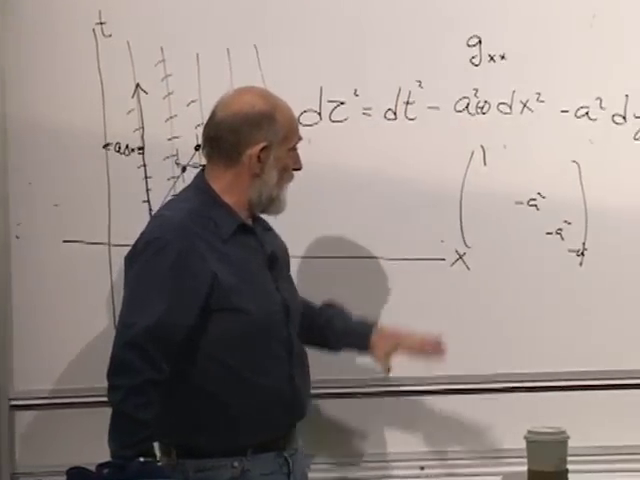
\includegraphics[width=0.82\textwidth]{lecture_01_figure_02.png}\caption{팽창하는 1차원 우주의 동행 세계선과 이에 대응하는 시공간 간격.}\end{figure}

세 공간 차원에서는 같은 양상을 바탕으로 신중하게 다음과 같이 확장할 수 있다.\footnote{판서의 일부는 00:56:38--00:58:51 무렵 가려져 있다. 이 세 차원 형태는 한 공간 차원에서 세 공간 차원으로 확장한다는 설명과 판서에 보이는 대각선 패턴을 함께 따른다.}
\begin{equation}
d\tau^2=dt^2-a^2(t)\bigl(dx^2+dy^2+dz^2\bigr),
\end{equation}
대각 계량은 다음과 같이 주어진다.
\begin{equation}
g_{\mu\nu}=\mathrm{diag}\bigl(1,-a^2,-a^2,-a^2\bigr).
\end{equation}
비대각 성분은 사라진다.
\begin{equation}
g_{tx}=g_{ty}=g_{tz}=0.
\end{equation}

균질성이란 계량 계수들이 시간에는 의존할 수 있지만 공간상의 위치에는 의존하지 않는다는 뜻이다. 등방성이란 세 공간 방향이 같은 방식으로 들어간다는 뜻이다.

\begin{classroomqa}\audiencequestion{\(dx\)를 거리라고 생각해야 하는 것 아닌가요?}\lecturetimestamp{01:01:18}\lecturerresponse{아닙니다. \(dx\)는 거리가 아닙니다. \(a\,dx\)가 거리입니다. \(dx\)는 단지 좌표 간격입니다. 이를 이해하는 한 가지 좋은 방법은 누군가 어느 순간 은하들 사이에 좌표 격자를 그린 다음 그 격자가 은하들을 따라가도록 정했다고 상상하는 것입니다. 그렇게 정했으므로 좌표 간격은 고정되어 있지만 물리적 거리는 변합니다. 거리 단위를 \(x\) 대신 \(a\)에 넣어도 됩니다. 이는 관례의 문제입니다. 중요한 것은 곱 \(a\,dx\)입니다.}\end{classroomqa}

\begin{classroomqa}\audiencequestion{\(dt^2\)의 계량 계수가 \(1\)과 같습니다. 이것도 단지 관례인가요?}\lecturetimestamp{01:03:24}\lecturerresponse{네. 그 자체로는 물리적인 의미가 없습니다. 계수가 시간에만 의존한다면 시간 변수를 바꾸어 그 계수를 단순히 \(dt^2\)로 만들 수 있습니다. 마찬가지로 \(c=1\)인 단위를 택할 수도 있습니다. 여기서 관례가 아닌 것은 계수가 위치에는 의존하지 않는다는 점입니다. 다만 시간에는 의존할 수 있습니다.}\end{classroomqa}

\begin{classroomqa}\audiencequestion{이것을 아인슈타인 장방정식에 넣으면 에너지-운동량 텐서는 어떻게 되나요?}\lecturetimestamp{01:05:59}\lecturerresponse{그것은 다음 종류의 질문이지만, 지금 논의하는 내용이 아니라 동역학에 속합니다. 이 계량을 아인슈타인 방정식에 넣고 어떤 에너지-운동량 분포가 해를 만들지 물을 수 있습니다. 아주 중요한 문제지만, 지금 다루는 주제는 동역학이 아니라 기하학입니다.}\end{classroomqa}

\section{지평선이 가리는 것}

큰 규모의 우주가 균질하고 등방적이라는 가정은 근사적으로만 다룬다. 별이나 행성, 심지어 개별 은하의 규모에서 우주는 분명 균질하지 않다. 국소적인 관측에서도 정확히 등방적이지는 않다.

농부의 밭을 생각하면 규모에 따른 차이를 이해할 수 있다. 한 규모에서는 규칙적으로 보이지만, 훨씬 작은 규모에서는 분명 그렇지 않다. 밭 전체보다 더 큰 규모에서는 다시 균질해 보이지 않는다. 우주론도 마찬가지다. 많은 은하에 대해 평균을 내면 큰 규모의 분포는 대략 균일해 보인다. 충분히 작은 규모에서는 그렇지 않다.

우주는 우리가 볼 수 있는 영역보다 크고, 우리가 앞으로도 볼 수 있는 영역보다 크다. 실제로 탐사할 수 있는 규모에서 우주는 국소적인 변화를 제외하면 등방적이고 균질하다. 그 바깥에 대해서는 직접 관측으로 보장되는 것이 없다.

\begin{classroomqa}\audiencequestion{우리가 정말 직접 알아낼 수는 없다고 하셨는데요. 그렇다면 간접적으로 알아낼 방법은 있을 수도 있나요?}\lecturetimestamp{01:10:34}\lecturerresponse{그럴 수도 있습니다. 요즘에는 충분히 큰 규모에서 우주가 균질하지 않다고 보는 견해가 대부분이며, 저도 그렇게 생각합니다. 하지만 제가 이 내기를 이기지도 지지도 않을 거라고 봅니다. 근본적이고 기본적인 이유 때문에 지금 볼 수 있는 곳보다 훨씬 더 멀리 볼 수는 없기 때문입니다. 지평선이 존재한다는 것이 바로 그 이유입니다.}\end{classroomqa}

\begin{classroomqa}\audiencequestion{중력을 이용하면 보이지 않는 곳 너머의 질량을 찾아낼 수 있지 않나요?}\lecturetimestamp{01:11:53}\lecturerresponse{아닙니다. 멀리 있는 질량은 우리를 단지 자유낙하 상태로 만들 수도 있습니다. 창문 없는 방에 앉아 있는 우리는 태양의 중력장 안에서 태양 주위를 공전하지만, 밖을 보지 못한다면 태양이 있다는 사실을 알아내기 어렵습니다. 조석력만이 태양의 존재를 드러내며, 원천이 충분히 멀리 있으면 그 조석 효과는 너무 작아 감지할 수 없을 수도 있습니다.}\end{classroomqa}

따라서 지평선은 직접 지식에 대한 궁극적인 장벽이다. 그는 우주의 부피가 우리가 앞으로도 볼 수 있는 영역의 부피보다 적어도 천 배는 크다고 사실상 확신하면서 말하고, 그 주장의 이유는 나중으로 미룬다.

\section{경계 없이 유계인 공간}

이제 닫힌 기하학을 살펴보자. 무한 직선은 열려 있고 비유계다. 선분은 범위가 유한하다는 의미에서 유계다. 유계라는 말은 경계가 있다는 뜻이 아니라 범위가 유한하다는 뜻이다.

벽이 있는 정육면체는 적절한 예가 아니다. 벽 가까이에 있는 사람과 벽에서 먼 사람은 동등하지 않으므로 균질성을 위배한다. 중심에 있는 사람조차 방향에 따라 다른 것을 보므로 등방성도 위배한다.

원이나 공의 내부도 적절하지 않다. 중심에 있는 사람은 모든 방향에서 같은 것을 보지만, 그런 대칭성을 지닌 곳은 특별한 한 점뿐이다. 중심에서 벗어나면 한 방향으로는 벽이 가깝고 다른 방향으로는 멀다. 따라서 일반적인 관측자에게 공간은 균질하지도 등방적이지도 않다.

아주 큰 규모에서는 우주가 균질하고 등방적이라는 가정을 기본으로 삼는다. 이것이 우주론적 원리다. 유용한 가정이지만 수정될 가능성에서 자유롭지는 않다.

\begin{classroomqa}\audiencequestion{모든 곳에서 등방적이면 균질하다는 뜻인가요?}\lecturetimestamp{01:18:57}\lecturerresponse{네. 모든 관측자가 모든 방향에서 같은 것을 본다면 균질성도 따른다는 뜻입니다. 그러나 그 역은 성립하지 않습니다. 균질하다고 해서 등방적인 것은 아닙니다. 예를 들어 우주 전체에 화살표가 모두 같은 방향을 가리키며 차 있다고 하면, 우주는 균질하면서도 선호되는 방향을 가질 수 있습니다.}\end{classroomqa}

적절한 유계 모형은 아무 특징도 없는 구의 표면이다. 그 표면에 갇혀 사는 2차원 생명체에게는 세계가 유한한데도 모든 장소가 국소적으로 서로 같고 모든 방향도 서로 같다. 이것이 경계 없이 유한한 공간이다.

\section{원 위의 닫힌 1차원 우주}

대수를 단순하게 하려고 구의 예를 한 공간 차원으로 줄여 원 위에서 살아가는 경우를 생각하자. 1차원에서 등방성은 왼쪽과 오른쪽이 동등하다는 뜻이다. 원은 정확히 그런 성질을 지닌다. 한 점을 택해 \(\theta=0\)라고 하자. 나머지 모든 점은 라디안으로 측정한 각좌표 \(\theta\)로 표시한다. 원점 바로 한쪽에 있는 점은 작은 음의 각도로도, \(2\pi\)에 조금 못 미치는 각도로도 나타낼 수 있다. 이러한 주기성은 기하학의 일부다.

원 위의 거주자들이 다룰 수 있는 것은 원주뿐이며, 바깥쪽의 반지름이나 중심은 대상이 아니다. 원을 따라 걸어 처음 출발한 점으로 돌아올 때까지 이동하면 전체 길이를 잴 수 있다. 원을 주변의 평면에 그리면 반지름과 비슷한 양을 도입할 수도 있지만, 그것은 매장 그림에 속하며 그들이 재는 내재적 기하학에는 속하지 않는다.

여기서 칠판 그림은 각도 좌표와 전체 원주를 한 그림에 보여 주므로 유용하다.
\begin{figure}[H]\centering
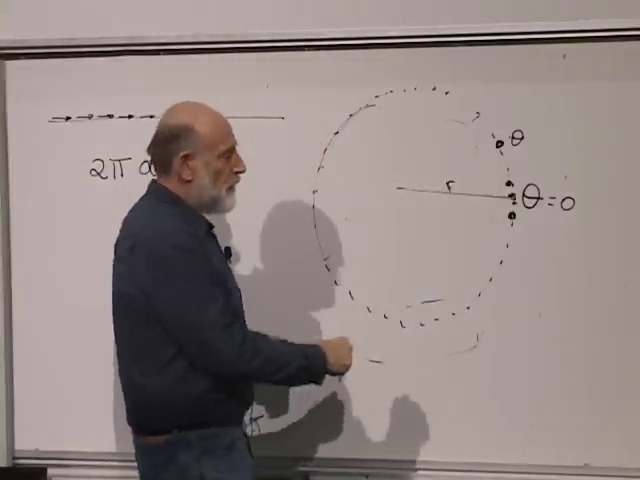
\includegraphics[width=0.82\textwidth]{lecture_01_figure_03.png}\caption{전체 원주가 \(2\pi a\)인 닫힌 1차원 우주의 각도 표현.}\end{figure}

편리한 관례는 다음과 같다.\footnote{01:26:40--01:29:20 주변에서는 전체 원주 자체를 척도인자로 놓는 경우와 이를 \(2\pi a\)로 쓰는 경우가 잠시 혼용된다. 뒤의 관례가 호 길이 공식으로 이어지는 표기이므로 여기서는 이를 사용한다.}\begin{equation}
L=2\pi a,
\end{equation}여기서 \(L\)는 전체 원주다.

작은 각도 간격 \(\Delta\theta\)에 대해 물리적 거리는
\begin{equation}
d=a\,\Delta\theta.
\end{equation}
무한소로 가면
\begin{equation}
ds=a\,d\theta,
\end{equation}
따라서
\begin{equation}
ds^2=a^2\,d\theta^2.
\end{equation}
이것이 원 위의 국소 계량이다.

\(a\)가 시간에 따라 변하면 닫힌 1차원 우주는 팽창하거나 수축한다. 고정된 은하 쌍에 대해
\begin{equation}
d(t)=a(t)\,\Delta\theta,
\end{equation}
따라서
\begin{equation}
\dot d=\dot a\,\Delta\theta
      =\frac{\dot a}{a}\,d.
\end{equation}
여기에서도 허블 법칙은 성립한다. 다만 원의 반대쪽으로 가는 경로가 모호해질 정도로 멀리 떨어지지 않은 은하 쌍에 한해서다.

시공간 계량은 다음과 같다.
\begin{equation}
d\tau^2=dt^2-a^2(t)\,d\theta^2.
\end{equation}
\(a\)가 일정하면 시공간 그림은 원기둥이다. \(a\propto t\)이면 원뿔이다. \(a(t)\)가 더 불규칙하게 변하면 그림은 꽃병 모양이 된다.

그림을 거꾸로 따라가면 은하들이 점점 더 가까워진다. 원주를 따라 \(360\)개의 은하가 있다고 하면, 나중에는 서로 널찍이 퍼져 있고 더 이른 때에는 아주 가까워지며, 그보다 더 이른 때에는 더욱 가까워진다. 결국 은하들은 더 이상 서로 분리된 은하가 아니게 되고, 그보다 더 이른 때에는 서로 분리된 원자조차 아니게 된다. 그래도 공간의 특별한 점은 없다.

이 모형에서 빅뱅이 어디에서 일어났는가라는 질문에 가장 명확히 답하면 이렇다. \(a(t)\to 0\)일 때 모든 두 점 사이의 거리 \(a(t)\,\Delta\theta\)는 0으로 간다. 우주 전체가 모든 곳에서 동시에 작아진다. 은하들은 외부 공간의 특권적인 한 장소에서 날아가고 있는 것이 아니다. 기하학 자체의 척도가 변하고 있다. 그런 의미에서 답은 어디에서나이다.

\begin{classroomqa}\audiencequestion{시공간이 휘어 있다고 하셨는데, 원기둥이라면 휘어 있나요?}\lecturetimestamp{01:38:04}\lecturerresponse{아닙니다. 원기둥이라면 휘어 있지 않습니다. 이 경우에는 \(a\)가 시간에 따라 일정합니다. 더 높은 차원의 공간에 그려져 있어서 휘어 보일 뿐입니다. 원기둥을 잘라 펼치면 늘이지 않고도 평평하게 놓을 수 있습니다.}\end{classroomqa}

이어서 원뿔을 살펴보자. \(a\propto t\)이면 시공간 그림은 원뿔이다. 원뿔의 꼭짓점에서 떨어진 부분도 같은 내재적 의미에서 평평하다. 펼쳐서 평면으로 만들 수 있다. 꼭짓점은 다르다. 그곳은 원뿔 특이점이다.

다음 단계에서는 구형 우주의 기하학을 살펴본 뒤, \(a(t)\)가 어떻게 커지거나 작아지는지 결정하는 동역학을 다룬다.